\documentclass[t]{beamer}
\usepackage[]{graphicx}
\usepackage[table]{xcolor}
\makeatletter
\def\maxwidth{%
  \ifdim\Gin@nat@width>\linewidth
    \linewidth
  \else
    \Gin@nat@width
  \fi
}
\makeatother

\definecolor{fgcolor}{rgb}{0.345, 0.345, 0.345}
\newcommand{\hlnum}[1]{\textcolor[rgb]{0.686,0.059,0.569}{#1}}%
\newcommand{\hlsng}[1]{\textcolor[rgb]{0.192,0.494,0.8}{#1}}%
\newcommand{\hlcom}[1]{\textcolor[rgb]{0.678,0.584,0.686}{\textit{#1}}}%
\newcommand{\hlopt}[1]{\textcolor[rgb]{0,0,0}{#1}}%
\newcommand{\hldef}[1]{\textcolor[rgb]{0.345,0.345,0.345}{#1}}%
\newcommand{\hlkwa}[1]{\textcolor[rgb]{0.161,0.373,0.58}{\textbf{#1}}}%
\newcommand{\hlkwb}[1]{\textcolor[rgb]{0.69,0.353,0.396}{#1}}%
\newcommand{\hlkwc}[1]{\textcolor[rgb]{0.333,0.667,0.333}{#1}}%
\newcommand{\hlkwd}[1]{\textcolor[rgb]{0.737,0.353,0.396}{\textbf{#1}}}%
\let\hlipl\hlkwb

\usepackage{framed}
\makeatletter
\newenvironment{kframe}{%
 \def\at@end@of@kframe{}%
 \ifinner\ifhmode%
  \def\at@end@of@kframe{\end{minipage}}%
  \begin{minipage}{\columnwidth}%
 \fi\fi%
 \def\FrameCommand##1{\hskip\@totalleftmargin \hskip-\fboxsep
 \colorbox{shadecolor}{##1}\hskip-\fboxsep
     \hskip-\linewidth \hskip-\@totalleftmargin \hskip\columnwidth}%
 \MakeFramed {\advance\hsize-\width
   \@totalleftmargin\z@ \linewidth\hsize
   \@setminipage}}%
 {\par\unskip\endMakeFramed%
 \at@end@of@kframe}
\makeatother

\definecolor{shadecolor}{rgb}{.97, .97, .97}
\newenvironment{knitrout}{}{} 

\usepackage{booktabs, textpos, multirow, array, amsmath, amsthm, Sweave}

\usetheme{Dresden}
\setbeamertemplate{headline}{
  \leavevmode%
  \hbox{%
    \begin{beamercolorbox}[wd=\paperwidth,ht=2.5ex,dp=1ex,left]{section in head/foot}
      \hspace*{1em}\insertsection
    \end{beamercolorbox}%
  }
}
\addtobeamertemplate{frametitle}{}{%
    \begin{textblock*}{1cm}(1.11\textwidth,1.105\textheight)
        \color{white}\tiny\insertframenumber{} / \inserttotalframenumber
    \end{textblock*}
}

% --- Presentation information ---
\title{Replication: Factor Momentum}
\subtitle{Based on Arnott, Kalesnik, \& Linnainmaa (2023)}
\author{Caterina Piancentini, Farkas Tallos, Giulio Iepure, Tomas Samaj}
\institute[WU Vienna]{ZZ ILab \\ WU Vienna}
\date{Term 2025/2026 -- ZZ QFin ILab Meeting 2}

\begin{document}

% --- Title Frame ---
{
\begin{frame}[plain]
    \titlepage
\end{frame}
}

% --- Table of Contents ---
\begin{frame}{Table of Contents}
    \tableofcontents
\end{frame}

% ============================
% SECTION 1: Papers and Context
% ============================
\section{Papers and Context}

\begin{frame}{Arnott, Kalesnik \& Linnainmaa (2023) -- \textit{Factor Momentum}}
\textbf{Main Idea:}
\begin{itemize}
    \item Extends momentum research to factor portfolios—showing that factor returns themselves exhibit momentum.
    \item Finds that factor momentum \textbf{subsumes} industry momentum.
    \item Uses principal component analysis to identify systematic sources of momentum.
\end{itemize}

\textbf{Key Insight:}
\begin{itemize}
    \item Momentum is strongest in high-eigenvalue factors explaining most of cross-sectional returns.
    \item Momentum arises from systematic components, not just stock-level trends.
\end{itemize}

\textbf{Relevance:} Our replication reproduces Appendix plots comparing factor and industry momentum.
\end{frame}

\begin{frame}{Ehsani \& Linnainmaa (2022) -- \textit{Factor Momentum and the Momentum Factor}}
\textbf{Contribution:}
\begin{itemize}
    \item Shows that momentum in stock returns stems from momentum in factor returns.
    \item Factors show strong autocorrelation: winners stay winners, losers stay losers.
\end{itemize}

\textbf{Interpretation:}
\begin{itemize}
    \item Momentum reflects timing of factor exposures, not a separate risk factor.
    \item Complements Arnott et al. (2023) by providing theoretical grounding.
\end{itemize}

\textbf{Link:} Our replication validates these findings using Fama–French and JKP datasets.
\end{frame}

\begin{frame}{AQR Alternative Trends UCITS Fund (2025) -- \textit{Practical Application}}
\textbf{Context:}
\begin{itemize}
    \item AQR’s trend-following fund applies cross-asset and factor momentum.
    \item Combines price-based and fundamental trend signals across global assets.
\end{itemize}

\textbf{Performance (Q1 2025 Report):}
\begin{itemize}
    \item Annualized return: 11.9\%; Sharpe ratio: 0.76.
    \item Low equity correlation (-0.20) and positive macro exposure.
\end{itemize}
\end{frame}

% ============================
% SECTION 2: Data
% ============================
\section{Data}

\begin{frame}{Outline}
    \tableofcontents[currentsection, hideallsubsections]
\end{frame}

\begin{frame}{Data Description}
\textbf{Datasets Used:}
\begin{itemize}
    \item \textbf{Fama–French 17 Industry Portfolios:} Monthly excess returns (July 1963–Dec 2024).
    \item \textbf{JKP Factors:} Cross-sectional factor returns (value, profitability, investment, quality, risk).
    \item \textbf{Thematic Factors:} Growth, leverage, volatility, and other economic themes.
\end{itemize}

\textbf{Data Processing:}
\begin{itemize}
    \item Cleaned and aligned to a common monthly sample.
    \item Standardized names and applied readable labels.
\end{itemize}

\textbf{Final Sample:} July 1963 – December 2024 (U.S. market).
\end{frame}

% ============================
% SECTION 3: Replication Methodology
% ============================
\section{Replication Methodology}

\begin{frame}{Outline}
    \tableofcontents[currentsection, hideallsubsections]
\end{frame}

\begin{frame}{Replication Methodology}
\textbf{Objective:} Replicate Arnott et al. (2023) Appendix figure comparing \textbf{Factor} vs. \textbf{Industry Momentum}.

\textbf{Strategy:}
\begin{enumerate}
    \item For each month:
    \begin{itemize}
        \item Rank all assets by previous month’s return.
        \item Go \textbf{long} the top half (winners), \textbf{short} the bottom half (losers).
    \end{itemize}
    \item Apply to Fama–French 17 industries and selected JKP factors.
    \item Equal-weight portfolios; rebalance monthly.
    \item Compute 1-month long–short return.
\end{enumerate}
\end{frame}

% ============================
% SECTION 4: Replication Results
% ============================
\section{Replication Results}

\begin{frame}{Outline}
    \tableofcontents[currentsection, hideallsubsections]
\end{frame}

\begin{frame}
\begin{knitrout}
\definecolor{shadecolor}{rgb}{0.969, 0.969, 0.969}\color{fgcolor}
\begin{figure}
{\centering 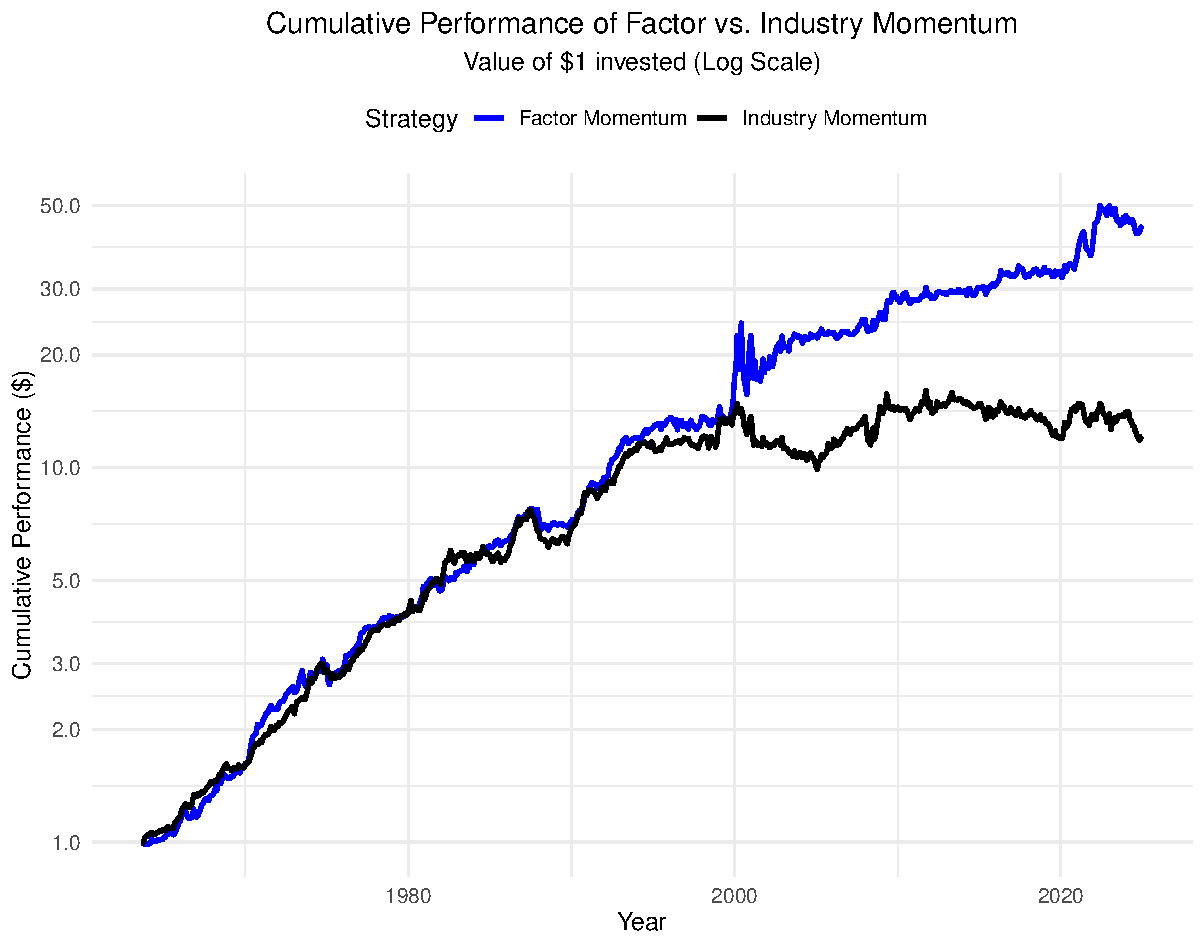
\includegraphics[width=\maxwidth]{figure/cum_ret_plot} }
\caption[Cumulative Performance (Log Scale), July 1963 - Dec 2024]{Cumulative Performance (Log Scale), July 1963 - Dec 2024}
\label{fig:cum_ret_plot}
\end{figure}
\end{knitrout}
\end{frame}

\begin{frame}
\begin{knitrout}
\definecolor{shadecolor}{rgb}{0.969, 0.969, 0.969}\color{fgcolor}
\begin{figure}
{\centering 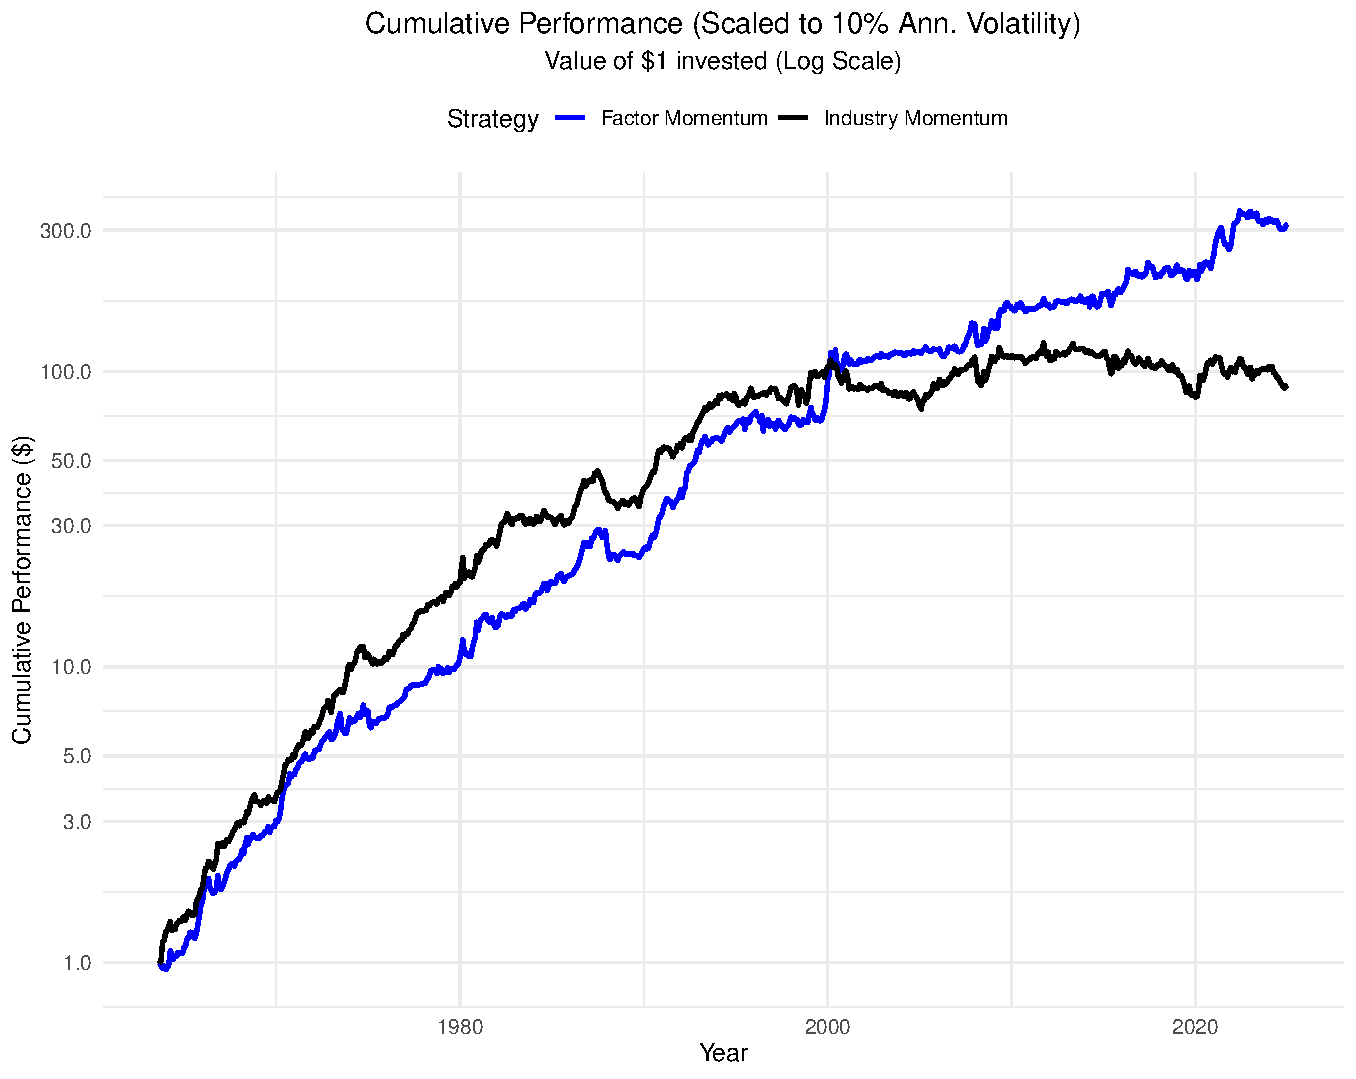
\includegraphics[width=\maxwidth]{figure/cum_ret_plot_vola_scaled} }
\caption[Cumulative Performance Vola Scaled (Log Scale), July 1963 - Dec 2024]{Cumulative Performance Vola Scaled (Log Scale), July 1963 - Dec 2024}
\label{fig:cum_ret_plot_vola_scaled}
\end{figure}
\end{knitrout}
\end{frame}

\begin{frame}{Arnott et al. (2023) Plot}
\begin{figure}[ht]
    \centering
    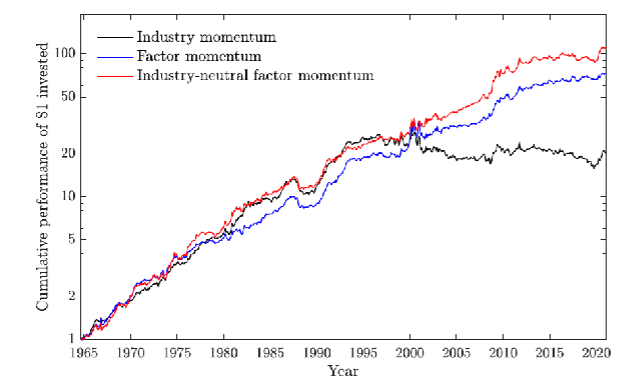
\includegraphics[width=0.92\linewidth]{Actual_plot.png}
    \caption{Industry vs. Factor vs. Industry-Neutral Factor Momentum (1965–2020).}
\end{figure}
\footnotesize
\textbf{Source:} Arnott, Kalesnik, Linnainmaa (2023), \textit{RFS}, 36(8), 3034–3070.
\end{frame}

% ============================
% SECTION 5: Factor Correlation Analysis
% ============================
\section{Factor Correlation Analysis}

\begin{frame}{Outline}
    \tableofcontents[currentsection, hideallsubsections]
\end{frame}

\begin{frame}{Factor Correlation Heatmap (Part 1)}
\textbf{Analysis:}
\begin{itemize}
    \item Correlation calculated among selected JKP factors.
    \item Helps identify relationships between factors being timed.
    \item \textbf{High correlations (dark green):}
    \begin{itemize}
        \item Strong among \textbf{profitability factors} — Gross Profitability, ROE, Profit Margin.
        \item \textbf{Investment factors} (Asset Growth, CAPX Growth) also highly correlated.
        \item Value-style factors moderately correlated with profitability.
    \end{itemize}
    \item Fundamental factors move together, reinforcing systematic momentum.
\end{itemize}
\end{frame}

\begin{frame}{Factor Correlation Heatmap (Part 2)}
\textbf{Analysis (continued):}
\begin{itemize}
    \item \textbf{Low/negative correlations (brown areas):}
    \begin{itemize}
        \item Distress and volatility proxies (Ohlson O-Score, Altman Z-Score, Residual Variance) have weak or negative links with profitability/value.
        \item Size (SMB) and momentum variables are largely orthogonal.
    \end{itemize}
    \item Indicates that some factors add \textbf{diversification} rather than reinforcement.
    \item Overall: Factor momentum mainly comes from \textbf{clusters of correlated, fundamental drivers}.
\end{itemize}
\end{frame}

\begin{frame}
\begin{knitrout}
\definecolor{shadecolor}{rgb}{0.969, 0.969, 0.969}\color{fgcolor}
\begin{figure}
{\centering 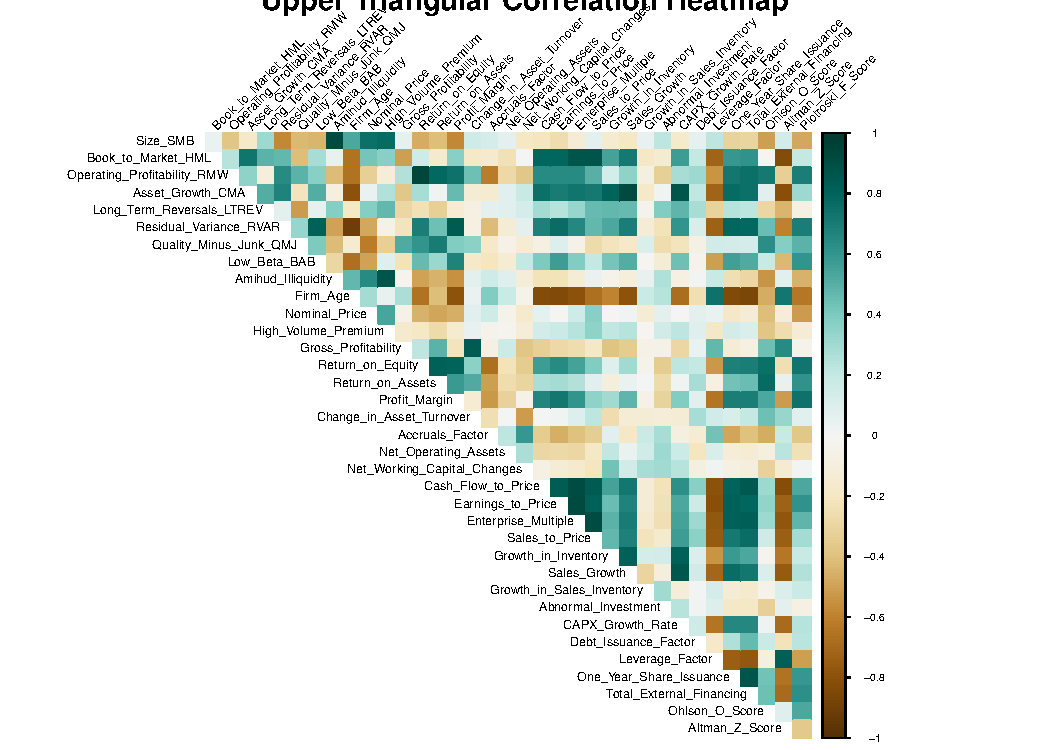
\includegraphics[width=\maxwidth]{figure/corr_heatmap1-1} }
\caption[Upper Triangular Correlation Heatmap of Selected JKP Factors]{Upper Triangular Correlation Heatmap of Selected JKP Factors}
\label{fig:corr_heatmap1}
\end{figure}
\end{knitrout}
\end{frame}

% ============================
% SECTION 6: Findings and Conclusion
% ============================
\section{Findings and Conclusion}

\begin{frame}{Outline}
    \tableofcontents[currentsection, hideallsubsections]
\end{frame}

\begin{frame}{Key Findings and Conclusion}
\begin{itemize}
    \item \textbf{Replication Findings:}
    \begin{itemize}
        \item Both industry and factor momentum strategies yield positive returns.
        \item Factor momentum appears stronger and more persistent, aligning with findings in the literature.
        \item The performance gap seems to widen in the extended sample period.
    \end{itemize}
    \item \textbf{Interpretation:}
    \begin{itemize}
        \item Factor momentum seems to subsume industry momentum, as suggested in the literature.
        \item \textbf{Correlation analysis identifies distinct clusters of fundamental drivers (e.g., Value, Profitability, Investment) suggesting systematic sources for factor momentum.}
    \end{itemize}
\end{itemize}
\end{frame}


\begin{frame}{Key Findings and Conclusion 2}
  \begin{itemize}
    \item \textbf{Conclusion:}
    \begin{itemize}
        \item Preliminary results support the hypothesis that short-term momentum is primarily driven by systematic factor dynamics rather than purely industry-specific effects.
    \end{itemize}
  \end{itemize}
\end{frame}




\begin{frame}{Next Steps: Refinement and Analysis}
    \vspace{0.5cm}
    \textbf{Deeper Analysis (Kickoff Goals):}
    \begin{itemize}
        \item \textbf{Factor Contribution Analysis:}
            \begin{itemize}
                \item Which factors drive the overall factor momentum return?
                \item \textbf{Further analyze the contribution of the identified factor clusters (Value, Profitability, Investment etc.) from the correlation analysis.}
            \end{itemize}
        \item \textbf{Factor Regressions:}
            \begin{itemize}
                \item Run regressions of individual JKP factors against FF3 / FF5+UMD models as requested in kickoff.
            \end{itemize}
        \item \textbf{Asset Allocation Context:}
            \begin{itemize}
                \item Calculate basic stats (Sharpe, Volatility) for the replicated Factor Momentum strategy.
                \item Identify the best strategies for potential inclusion in a broader asset allocation framework.
                \item Assess correlation with a standard 60/40 portfolio.
            \end{itemize}
    \end{itemize}

\end{frame}


\begin{frame}{Questions and Discussion Points}

    \textbf{Factor Set Alignment:}
    \begin{itemize}
        \item Our JKP dataset seems to align well, but we couldn't precisely match/find these factors from the RFS paper:
            \begin{itemize}
                \item \footnotesize Residual Variance, Sustainable Growth, Investment Growth Rate, Investment to Capital, Investment to Assets, Five-Year Share Issuance, Distress Risk, M/B Accruals.
            \end{itemize}
        \item Should we proceed with the current matched set (approx. 35 factors)? Does this significantly impact the replication?
    \end{itemize}
\end{frame}


\begin{frame}{Sneak Peek: Factor Regression Example}

    \textbf{Regression:} JKP `Book to Market HML` (Excess Return) FF3 Factors (MktRF + SMB + HML)

    \vspace{0.5cm}
    \textbf{Key Results:}
    \begin{itemize}
        \item \textbf{High HML Loading:} Coefficient on FF HML is 0.986 ($t = 36.8$), indicating the JKP factor strongly captures the standard value effect, as expected.
        \item \textbf{Significant Alpha:} The intercept is -0.41 percent per month ($t = -5.21$), suggesting the JKP HML factor underperformed the FF3 model's prediction.
        \item \textbf{SMB Exposure:} Significant negative loading on SMB (-0.108, t = -4.01), indicating a slight tilt towards larger stocks compared to the FF3 benchmark.
        \item \textbf{Model Fit:} The FF3 factors explain approx. 67 percent of the variance (Adj. R-squared = 0.666).
    \end{itemize}

    \vspace{0.5cm}
    \textit{Next step: Extend this analysis to all factors and additional models (FF5+UMD).}

\end{frame}


\begin{frame}[plain]
    \centering
    \vspace{2cm}
    {\Huge \textbf{Thank You}} \\[0.5cm]
    \Large Questions or comments? \\[1cm]
    \normalsize
    \textit{Replication of Arnott, Kalesnik, \& Linnainmaa (2023)} \\
    WU Vienna – ZZ QFin Lab 2025/26 
\end{frame}

\end{document}